
\subsection{M\'etodo de simulaciones}
\label{sec:simulacion}

Es dif\'icil identificar interacciones esenciales (PPIs) experimentalmente en la escala gen\'omica, dado que esta identificaci\'on requiere la demostraci\'on de que romper el enlace entre prote\'inas esenciales sin afectar otros aspectos de las funciones prote\'icas causa letalidad o infertilidad.

Aqu\'i usamos un m\'etodo computacional para evaluar la prevalecencia de enlaces esenciales PPIs y la contribuci\'on de PPIs esenciales a la esencialidad de genes al nivel gen\'omico.

Nuestro an\'alisis se enfoca en las redes {\it LIT} y {\it Y2H}.
%, excluyendo a la red {\it AP-MS}, como se hizo en la secci\'on anterior. 
%Tambi\'en excluimos a la red {\it LIT-Reguly} debido 

Como se mencion\'o antes, dos prote\'inas que forman un enlace esencial PPI deben ser esenciales.
Por el contrario, las interacciones entre prote\'inas esenciales (IBEPs, {\it Interaction Between Essential Proteins}, por sus siglas en ingl\'es) pueden o no ser esenciales, dado que la esencialidad de una prote\'ina puede deberse a otros factores adem\'as de las PPIs.
Esta caracter\'istica nos permite estimar el n\'umero de PPIs esenciales en una red, dado queque el n\'umero de IBEPs crece con el n\'umero de PPIs esenciales.

Dado el n\'umero total de interacciones IBEPs $N_{ie}$ para cada red, generamos una red de control haciendo un recableado de los enlaces, manteniendo la distribuci\'on de grado $P(k)$ para cada nodo.
Repitiendo este procedimiento 5000 veces (1000 para la red {\it Y2H}), obtenemos la distribuci\'on del n\'umero ($n_{ie}$) de enlaces esenciales (IBEPs) en redes recableadas al azar.
En todos los caso, el m\'aximo valores de la distribuci\'on no supera el caso de la red real; es decir, $max(n_{ie}) < N_{ie}$ siempre.
Este exceso del caso real tambi\'en se observa en otros casos de PPIs de levadura y en PPIs de nematodos {\bf CITAR 14 y 15, ver p. 2}.

Siguiendo el m\'etodo de \cite{he2006}, determinamos la fracci\'on de interacciones esenciales PPI como $\alpha = (N_{ie} - <n_{ie}>)/(N_{nod})$, siendo $N_{tot}$ el n\'umero total de nodos de la red.
Los valores para las diferentes redes se muestran en la tabla \ref{tab:probas}.


%--- overlapping
% NOTE: sacado de:
% ./beta -- ...
Notar que algunos nodos resultaron afectados por ambos factores; es decir por asignaci\'on random y por PPIs esenciales. 
En particular, para el caso {\it Y2H} es del $22 \pm 6$ \%, y para {\it LIT} es del $7.10 \pm 3.04$.

\begin{figure}
\centering
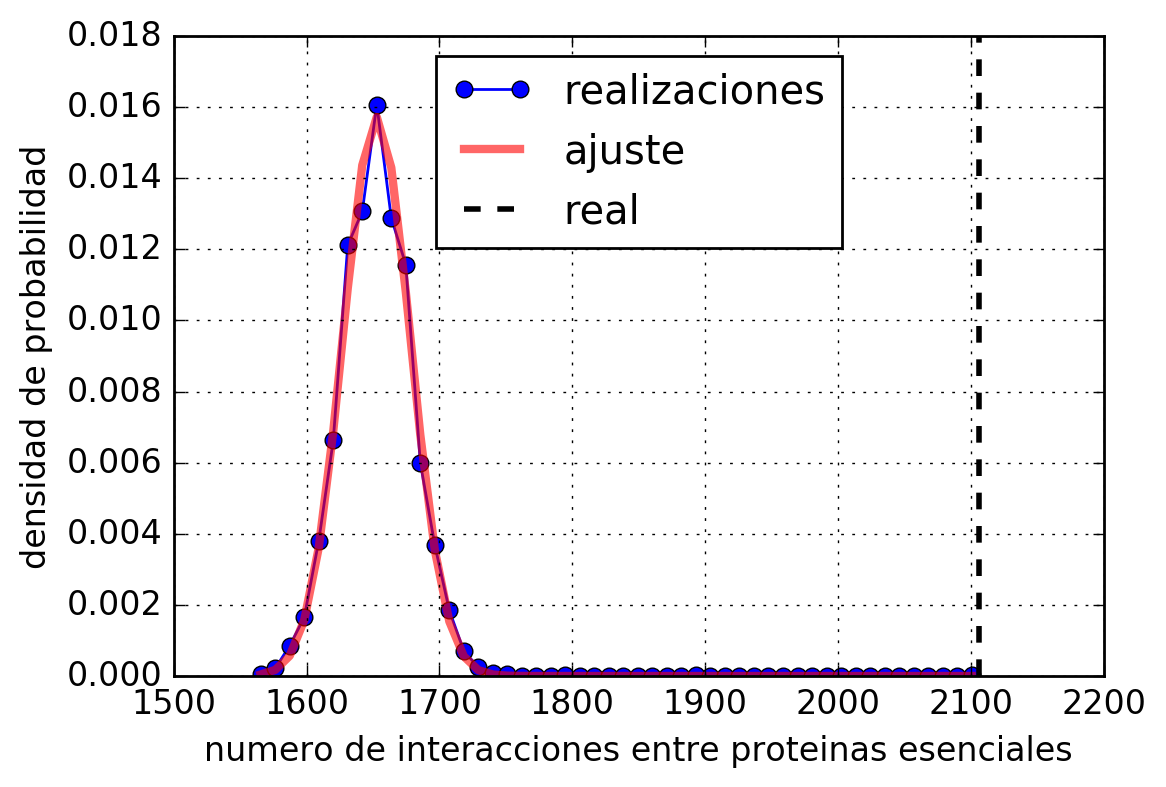
\includegraphics[scale = 0.6]{figuras/hist_LIT} 
\includegraphics[scale = 0.6]{figuras/hist_Y2H} \\
\caption{Distribuciones observadas del n\'umero de interacciones esenciales para los casos random de la redes estudiadas mediante simulaciones, para investigar las probabilidad $\alpha$ y $\beta$ de la red.}
\label{fig:remocion_alternativo}
\end{figure}

%EO
